\section{Implementation}\label{sec:implementation}

This section goes into the details of the implementation of the Simulink plant
and Python controller setup.

A high-level view of the setup is presented in Figure~\ref{fig:setup_diagram}.
The Simulink model's main responsability is running the CARNOT simulation. It
also has the task of providing the \acrshort{mpc} with information on the
weather forecast, since the weather information for the simulation comes from a
CARNOT \acrshort{wdb} object. A detailed view of all the information available
in the \acrshort{wdb} object is given in Section~\ref{sec:CARNOT_WDB}.


\begin{figure}[ht]
    \centering
    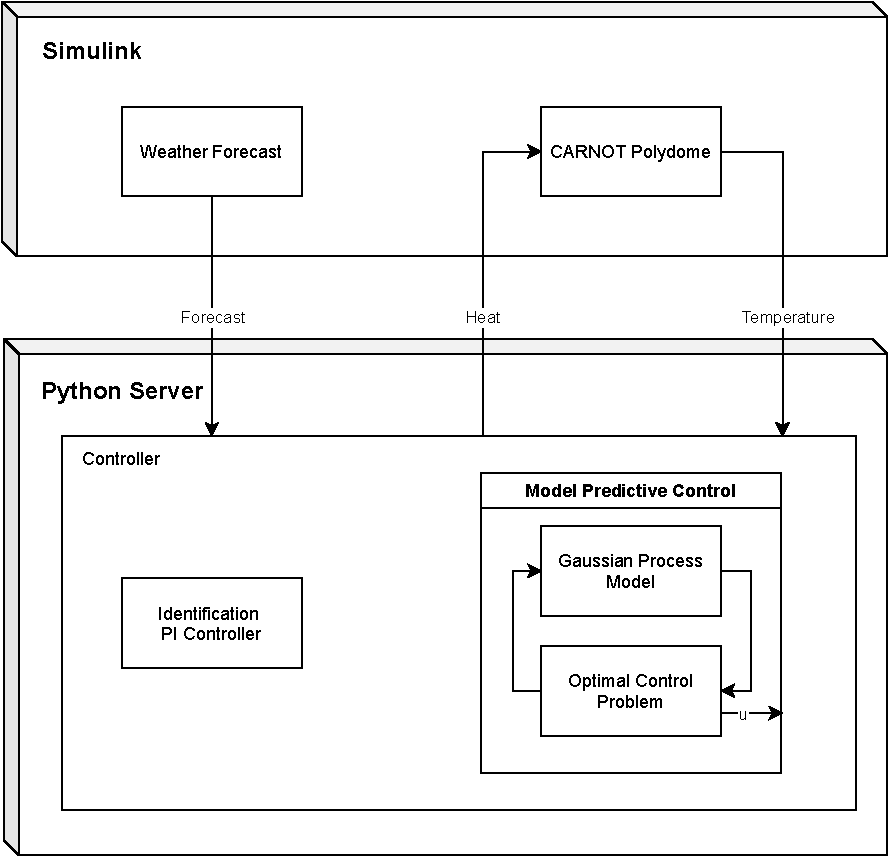
\includegraphics[width = 0.5\textwidth]{Images/setup_diagram.pdf}
    \caption{Block diagram of the Simulink plant and Python Controller}
    \label{fig:setup_diagram}
\end{figure}

\subsection{Simulink Model}

The secondary functions of the Simulink model is the weather prediction, as well
as communication with the Python controller. A complete schema of the Simulink
setup is presented in Figure~\ref{fig:Simulink_complete}.

\begin{figure}[ht]
    \centering
    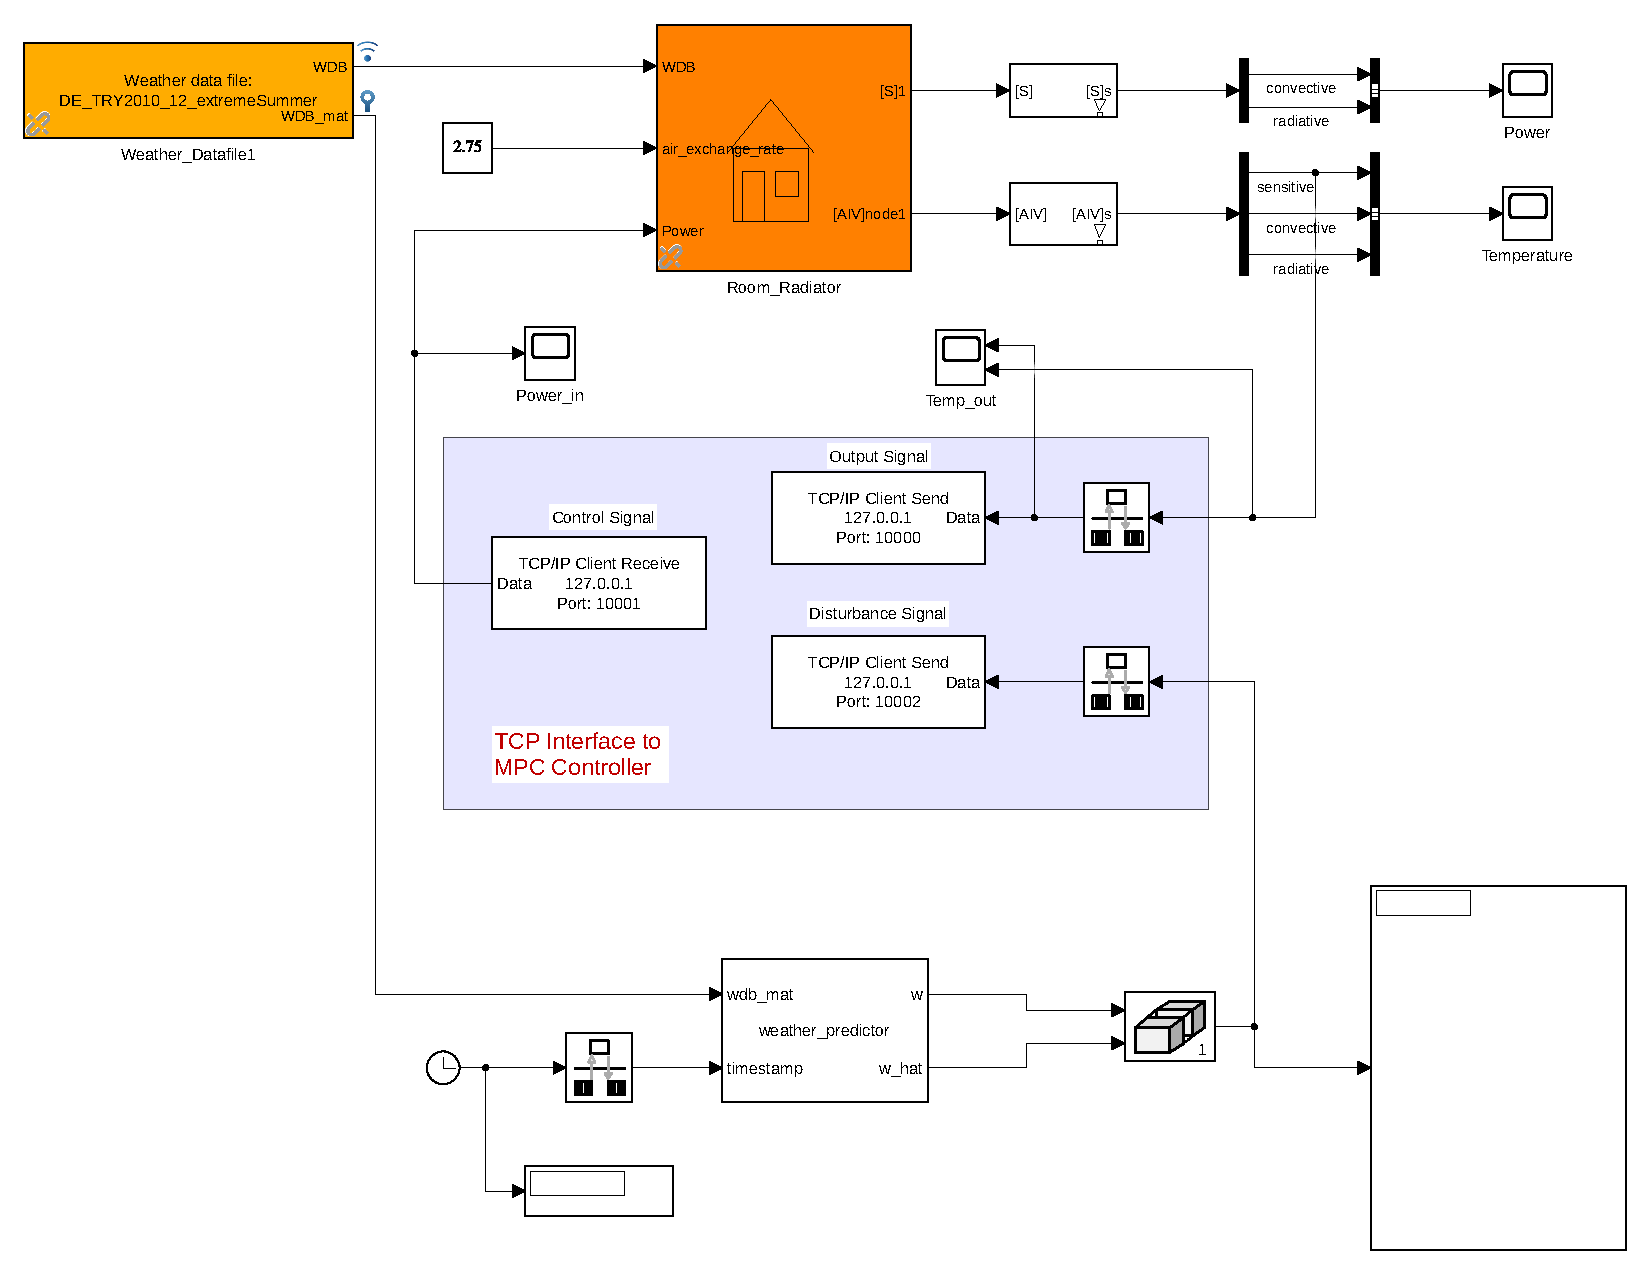
\includegraphics[width = 0.75\textwidth]{Images/polydome_python.pdf}
    \caption{Simulink Schema of the Complete Simulation}
    \label{fig:Simulink_complete}
\end{figure}

The communication between Simulink and the controller is done using three
separate TCP/IP sockets: one for sending the control signal, one for reading the
temperature measurement, and one for reading the weather forecast. This is
mainly due to a Simulink limitation which can only transfer one signal over a
single socket. This implementation also has the benefit of providing an
additional layer of abstraction for the controller and the controlled plant: as
long as the measurements, the actuators and the weather prediction can
communicate over TCP, these elements can all be implemented completely
separately, which is much more similar to a real-life implementation.

With this structure, the only information received and sent by the Python
controller is the actual sampled data, without any additional information. And
while the controller needs information on the control horizon in order to read
the correct amount of data for the weather predictions and to properly generate
the optimization problem, the discrete/continuous transition and vice-versa
happens on the Simulink side. This simplifies the adjustment of the sampling
time, with the downside of harder inclusion of meta-data such as hour of the
day, day of the week, etc.\ in the \acrlong{gp} Model.

The weather prediction is done using the information present in the CARNOT
\acrshort{wdb} object. Since the sampling time and control horizon of the
controller can be adjusted, the required weather predictions can lie within an
arbitrary time interval. At each sampling point, the weather measurements are
linearly interpolated for the span of time ranging from the most recent
measurement to the next measurement after the last required prediction time.
This provides a better approximation that pure linear interpolation over the
starting and ending points, while retaining a simple implementation.

\subsection{Gaussian Processes}

As described in Section~\ref{sec:gaussian_processes}, both training and
evaluating a \acrshort{gp} has an algotirhmic complexity of $\mathcal{O}(n^3)$.
This means that naive implementations can get too expensive in terms of
computation time very quickly.

In order to have as smallest of a bottleneck as possible when dealing with
\acrshort{gp}s, a very optimized implementation of \acrlong{gp} Models was
used, in the form of GPflow~\cite{matthewsGPflowGaussianProcess2017}. It is
based on TensorFlow~\cite{tensorflow2015-whitepaper}, which has very efficient
imeplentation of all the necessary Linear Algebra operations. Another benefit of
this implementation is the very simple use of any additional computational
resources, such as a GPU, TPU, etc.

\subsubsection{Classical Gaussian Process training}

For the training of the classical \acrshort{gp} models, the Scipy optimizer
provided by GPflow was used. By default, it uses the `L-BFGS-B' optimization
method, which runs until a local minimum of the negative log likelihood is
found. Since in the present implementation the \acrshort{gp} models are trained
only once, with a small amount of initial data, this approach was not only
sufficient, but also faster than the more complex implementation of training
used for \acrshort{svgp} models.

\subsubsection{Sparse and Variational Gaussian Process training}

The \acrshort{svgp} models have a more involved oprimization procedure due to to
several factors. First, when training an \acrshort{svgp} model, the optimization
objective is the value of the \acrshort{elbo} (cf. Section~\ref{sec:elbo}).
After several implementations, the more complex \textit{Adam} optimizer turned
out to provide much faster convergence compared to other optimizers. Second, in
the case of updating the model once per day with all the historical information,
the training dataset keeps getting larger each time. In order to combat this,
the sparse model was trained on minibatches of 1000 datapoints for 10000
iterations. Evaluating the \acrshort{elbo} on minibatches provide an unbiased
estimate of the actual value, given enough training iterations. This
implementation has the benefit of taking constant training time, which becomes
important later in the simulation, where the training dataset is much larger
than the initial amount of data.  

\subsection{Optimal Control Problem}

The \acrlong{ocp} has been implemented using the
CasADi~\cite{anderssonCasADiSoftwareFramework2019} algorithmic differentiation
framework. It provides an interface between a high-level definition of the
optimization problems, and the very efficient low-level solvers. 

The implementation of the \acrshort{ocp} defined in
Equation~\ref{eq:optimal_control_problem} has a few particularities, discussed
in the following subsections.

\subsubsection{Integrating GPflow models in CasADi}

The first particularity of the implementing the \acrshort{ocp} with CasADi is
the use of the CasADi callback objects. The purpose of these objects is
integration of external functions into CasADi. Generally, using callbacks is not
advised because each call to the external function incurs additional overhead.
These callbacks usually can't directly provide information on the
forward/reverse sensitivities, used by CasADi to drastically reduce computation
time. In the absence of this information, CasADi has to do many evaluations
around a point in order to approximate the gradients. TensorFlow keeps track of
all the computational graph's gradients, which can be accessed at a cost
slightly higher than the evaluation cost of the function.

Integrating the gradient information into the CasADi callbacks reduces the
number of function calls by around an order of magnitude, which already
drastically reduces computation time.

Another significant speed improvement comes from transforming the Python calls
to TensofFlow into native tf-functions. This change incurs a small overhead the
first time the optimization problem is run since all the TensorFlow functions
have to be compiled before execution, but afterwards speeds up the execution by
around another order of magnitude.

The last optimization done to the CasADi implementation is the use of the MA27
linear solver provided by the HSL optimization
library~\cite{HSLCollectionFortran}. This change results in an speedup of around
10\% compared to using the default MUMPS solver. While not as drastic as the
other improvements, this still provides a significant reduction in the runtime
of the whole year simulation.

\subsubsection{Sparse Implementation of the Optimization Problem}

The optimization problem as presented in
Equation~\ref{eq:optimal_control_problem} becomes very nonlinear quite fast. In
fact, due to the autoregressive structure of the \acrshort{gp}, the predicted
temperature at time t is passed as an input to the model at time $t+1$. A simple
recursive implementation of the Optimization Problem becomes untractable after
only 3 --- 4 prediction steps. 

In order to solve this problem, a new OCP is introduced. It has a much sparser
structure, in exchange for a larger number of variables. This turns out to be
much faster to solve than the original problem.

Let $w_l$, $u_l$, and $y_l$ be the lengths of the state vector components
$\mathbf{w}$, $\mathbf{u}$, $\mathbf{y}$ (cf. Equation~\ref{eq:components}).
Also, let X be the matrix of all the system states over the optimization horizon
and W be the matrix of the predicted disturbances for all the future steps. The
original \acrlong{ocp} can be rewritten as:

\begin{subequations}\label{eq:sparse_optimal_control_problem}
    \begin{align}
        & \text{minimize}
        & & \sum_{i=2}^{N + 1} \left(X[i, w_l + u_l + 1] - y_{ref, t}\right)^2 \\
        & \text{subject to}
        & & X[i+1, w_l + u_l + 1] = K_*K^{-1}X[i, :] \quad \text{for} \quad
        i\in[1, N]\\
        &&& X[i, w_l + u_l + 2: ] = X[i, w_l+ u_l + 1: w_l + u_l + y_l - 1]\\
        &&& X[i, 1:w_l] = W[i, :] \\
        &&& X[i+1, w_l + 2: w_l + u_l] = X[i, w_l + 1: w_l + u_l - 1] \\
        &&& X[:, w_l + 1] \in \mathcal{U}
    \end{align}
\end{subequations}

\subsection{Python server}

The Python server is responsible for the control part of the simulation. It
delegates which controller is active, is responsible for training and updating
the \acrshort{gp} and \acrshort{svgp} models, as well as keeping track of all
the intermediate results for analysis.

In the beginning of the experiment there is no information available on the
building's thermal behaviour. For this part of the simulation, the controller
switches to a \acrshort{pi} controller until it gathers enough data to train a
\acrshort{gp} model. The signal is then disturbed by a random signal before
being applied to the CARNOT building. This ensured that the building is
sufficiently excited to capture its dynamics, while maintaining the
temperature within an acceptable range (~15 --- 25 $\degree$C).

Once enough data has been captured, the Python controller trains the
\acrshort{gp} model and switches to tracking the appropriate SIA 180:2014
reference temperature (cf. Section~\ref{sec:reference_temperature}).

For the case of the \acrshort{svgp}, a new model is trained once enough data is
gathered. The implementations tested were updated once a day, either on the
whole historical set of data, or on a window of the last five days of data.

\clearpage
